\documentclass[11pt,a4paper]{article}
\usepackage[margin=2.5cm]{geometry}
\usepackage{amsmath,amssymb}
\usepackage{graphicx}
\usepackage{listings}
\usepackage{xcolor}
\usepackage{hyperref}
\usepackage{booktabs}

\lstset{basicstyle=\ttfamily\small, breaklines=true, frame=single,
        backgroundcolor=\color{gray!8}, language=Python, keywordstyle=\color{blue!60!black}}

\begin{document}

\begin{titlepage}
\centering
\vspace*{0.5cm}
\includegraphics[width=3.6cm]{figures/logo.png}\\[0.6cm]
{\LARGE\bfseries AIN SHAMS UNIVERSITY}\\[0.25cm]
{\Large\bfseries FACULTY OF ENGINEERING}\\[0.2cm]
{\large i-Credit Hours Engineering Programs}\\[0.1cm]
{\normalsize Computer and Artificial Intelligence Engineering}\\[0.3cm]
\rule{\textwidth}{0.8pt}\\[1.6cm]

{\Large Course Code: \textbf{CSE488}}\\[0.3cm]
{\huge\bfseries Deep Learning}\\[1.4cm]

{\LARGE\bfseries Assignment 1}\\[0.3cm]
{\Large MicroGrad (Scalar Autograd Engine)}\\[0.5cm]
{\large Documentation Report}\\[2.2cm]

\begin{tabular}{rl}
\large\textbf{Student Name:} & \large Abdelrahman Mohamed Bahig \\[0.4cm]
\large\textbf{Student ID:}   & \large 23P0390 \\[0.4cm]
\large\textbf{Course:}       & \large CSE488 -- Deep Learning \\[0.4cm]
\large\textbf{Date:}         & \large \today \\
\end{tabular}

\vfill
\rule{\textwidth}{0.8pt}\\[0.2cm]
{\small Faculty of Engineering, Ain Shams University}
\end{titlepage}

\tableofcontents
\newpage

\section{Overview}
This report documents a from-scratch scalar automatic differentiation engine (\texttt{src/engine.py}), a small neural network API built on it (\texttt{src/nn.py}), the course test suites (\texttt{tests/test\_engine.py}, \texttt{tests/test\_nn.py}), and a demo notebook (\texttt{demo.ipynb}). No PyTorch or other autograd library is used; only the Python standard library inside the engine, and NumPy/Matplotlib in the notebook for data and plots.

\section{Mathematical Derivations}
\subsection{Reverse-mode automatic differentiation}
Every arithmetic operation creates a node in a directed acyclic graph (DAG). Let $L$ be the final scalar output and $v$ any intermediate node. Reverse-mode accumulates $\bar v := \partial L/\partial v$. For a node $y = f(x_1,\dots,x_k)$ the chain rule gives
\begin{equation}
\frac{\partial L}{\partial x_i} \mathrel{+}= \frac{\partial L}{\partial y}\cdot\frac{\partial y}{\partial x_i}.
\end{equation}
The update uses \texttt{+=} (accumulation) because a node may feed several consumers, and by the multivariate chain rule the total gradient is the \emph{sum} of the contributions from all consumers:
\begin{equation}
\frac{\partial L}{\partial x} = \sum_{y\,:\,x\in \mathrm{parents}(y)} \frac{\partial L}{\partial y}\frac{\partial y}{\partial x}.
\end{equation}

\subsection{Local derivatives}
\paragraph{Addition.} $y=a+b$: $\ \partial y/\partial a = \partial y/\partial b = 1$, hence $\bar a \mathrel{+}= \bar y,\ \bar b \mathrel{+}= \bar y$.

\paragraph{Multiplication.} $y=ab$: $\ \partial y/\partial a = b,\ \partial y/\partial b = a$, hence $\bar a \mathrel{+}= b\,\bar y,\ \bar b \mathrel{+}= a\,\bar y$.

\paragraph{Power (constant exponent).} $y=a^{n}$: $\ \partial y/\partial a = n\,a^{n-1}$, hence $\bar a \mathrel{+}= n\,a^{n-1}\,\bar y$. The exponent is restricted to a Python \texttt{int}/\texttt{float} constant, so no gradient flows to it.

\paragraph{Hyperbolic tangent.} $y=\tanh a = \dfrac{e^{a}-e^{-a}}{e^{a}+e^{-a}}$. Then
\[
\frac{dy}{da}=\frac{(e^a+e^{-a})^2-(e^a-e^{-a})^2}{(e^a+e^{-a})^2}=1-\tanh^2 a,
\]
hence $\bar a \mathrel{+}= (1-y^2)\,\bar y$. The derivative is expressed via the already-computed output $y$, so no extra evaluation is needed.

\paragraph{Exponential.} $y=e^{a}$: $\ dy/da=e^a=y$, hence $\bar a \mathrel{+}= y\,\bar y$.

\paragraph{Derived operators.} Negation is $a\cdot(-1)$; subtraction is $a+(-b)$; division is $a\cdot b^{-1}$. Their gradients therefore follow automatically from the three primitives. For instance, for $y=a/b$: $\partial y/\partial a = b^{-1}$ and $\partial y/\partial b = -a\,b^{-2}$, which the engine reproduces through \texttt{mul} and \texttt{pow} with $n=-1$ (values checked in \texttt{test\_basic\_operations}; gradients checked numerically in the notebook).

\subsection{Worked example}
For $L=\tanh(x_1w_1+x_2w_2+b)$ with $x_1=2,\ x_2=0,\ w_1=-3,\ w_2=1,\ b=6.8813735870195432$: the pre-activation is $n=0.8813735\ldots$, $L=\tanh n=0.7071$, $\partial L/\partial n = 1-L^2 = 0.5$. Therefore $\partial L/\partial x_1 = w_1\cdot0.5=-1.5$, $\partial L/\partial w_1 = x_1\cdot0.5=1.0$, $\partial L/\partial x_2 = 0.5$, $\partial L/\partial w_2=0$. The engine reproduces these values (checked in the notebook).

\section{Topological Sort and Backpropagation}
A node's gradient is complete only after \emph{every} consumer of that node has pushed its contribution. Equivalently, we must process nodes in an order where each node is handled before all of its inputs. A topological ordering of the DAG, reversed, provides exactly this.

\subsection{Algorithm}
\begin{lstlisting}
def _get_topo(self):
    topo, visited = [], set()
    def build_topo(node):
        if node not in visited:
            visited.add(node)
            for child in node._prev:
                build_topo(child)
            topo.append(node)      # post-order
    build_topo(self)
    return topo

def backward(self):
    topo = self._get_topo()
    self.grad = 1.0                # seed dL/dL = 1
    for node in reversed(topo):
        node._backward()
\end{lstlisting}
The submitted implementation uses an explicit stack instead of recursion (same post-order, same \texttt{visited} logic), so that very deep graphs do not exceed Python's recursion limit:
\begin{lstlisting}
def _get_topo(self):
    topo, visited = [], {self}
    stack = [(self, iter(self._prev))]
    while stack:
        node, children = stack[-1]
        for child in children:
            if child not in visited:
                visited.add(child)
                stack.append((child, iter(child._prev)))
                break
        else:
            topo.append(node)      # post-order: after all children
            stack.pop()
    return topo
\end{lstlisting}
\textbf{Correctness argument.} Appending a node \emph{after} recursing into all of its children (post-order) guarantees that every input appears in \texttt{topo} before any node that uses it. Reversing the list therefore visits every node before its inputs, so when \texttt{\_backward} of a node runs, its \texttt{grad} has already received the contributions of all of its consumers.

\subsection{TA traps and how the design avoids them}
\begin{itemize}
\item \textbf{Post-order trap.} If a node were appended \emph{before} its children were explored (pre-order), the reversed list could process an input before one of its consumers, which would push stale (incomplete) gradients. The composite test \texttt{test\_chain\_rule\_and\_backprop} checks the resulting gradients.
\item \textbf{Diamond graph trap.} For $c=a+a$ (or $c=a\cdot a$) the node $a$ is reachable by two paths. Without \texttt{visited}, $a$ is added twice and its backward runs twice (double counting); in a graph with deeper sharing the number of visits grows exponentially. With the set, $a$ appears once, and the two contributions are summed by \texttt{+=}, giving $\partial c/\partial a=2$ for $a+a$ and $2a$ for $a\cdot a$ (\texttt{test\_gradient\_accumulation\_diamond\_graph} checks that $d=(a+a)\cdot a$ gives $\partial d/\partial a=4a=12$).
\end{itemize}
The graph is a DAG by construction (a new node is built only from existing ones), so the DFS terminates. Because nodes are hashed by identity and no \texttt{\_\_eq\_\_} is overridden, two different nodes holding the same number are never confused.

\section{Neural Network API}
\begin{itemize}
\item \textbf{Neuron}: weights $w_i\sim U(-1,1)$ and bias $b\sim U(-1,1)$; output $\tanh(\sum_i w_ix_i+b)$. The sum is started from $b$ so the graph has no spurious constant node.
\item \textbf{Layer}: a list of \texttt{nout} neurons sharing the same input; returns a single \texttt{Value} when \texttt{nout}=1 and a list otherwise.
\item \textbf{MLP}: a chain of layers built from \texttt{[nin] + nouts}. For sizes $[n_0,n_1,\dots,n_L]$ the parameter count is $\sum_{l=1}^{L}(n_{l-1}+1)\,n_l$; for \texttt{MLP(3,[4,4,1])} this is $16+20+5=41$ (checked in \texttt{test\_mlp}).
\item \textbf{Parameters and gradients}: each class exposes \texttt{parameters()} and \texttt{zero\_grad()} (which calls \texttt{reset\_grad()} on every parameter). Gradients accumulate with \texttt{+=}, so \texttt{zero\_grad()} \emph{must} be called before every backward pass in a training loop.
\end{itemize}

\section{Design Justifications}
\begin{itemize}
\item \textbf{Closures for local derivatives.} Each operator stores a \texttt{\_backward} closure capturing its operands and output. This keeps the derivative rule next to its forward rule and avoids a large dispatch table keyed by operator name.
\item \textbf{Accumulation with \texttt{+=}.} Required for correctness on shared nodes (Section 3.2).
\item \textbf{Few primitives, many derived ops.} Only \texttt{add}, \texttt{mul}, \texttt{pow}, \texttt{tanh} and \texttt{exp} have hand-written derivatives; \texttt{neg}, \texttt{sub}, \texttt{div} and the reflected operators (\texttt{\_\_radd\_\_}, \texttt{\_\_rsub\_\_}, \texttt{\_\_rmul\_\_}, \texttt{\_\_rtruediv\_\_}) are compositions, minimizing the surface for bugs and letting expressions like \texttt{3 - a * 2 + 1 / a} work.
\item \textbf{Constants are wrapped in \texttt{Value}.} \texttt{a + 1} works without special cases; the wrapped constant simply receives an unused gradient.
\item \textbf{Iterative post-order DFS.} The hint's recursive DFS is correct but is limited by Python's recursion limit (about 1000 frames by default), which a long chain of operations would exceed. The engine therefore uses an explicit stack with the same post-order and \texttt{visited} logic; a chain of 20{,}000 additions was back-propagated without error (see the notebook).
\item \textbf{Verification strategy.} Three layers: analytic hand-derived values, graph-structure tests (the diamond graph), and numerical gradient checking by central differences $\frac{f(x+h)-f(x-h)}{2h}$ with $h=10^{-6}$ (error $\sim10^{-10}$ in the notebook).
\end{itemize}

\section{Test Results}
The course test suites (\texttt{tests/test\_engine.py} and \texttt{tests/test\_nn.py}) contain 12 tests; all pass (\texttt{python -m pytest -v}: \texttt{12 passed}).
\begin{center}
{\footnotesize
\begin{tabular}{p{7cm}p{8cm}}
\toprule
Test & What it checks \\
\midrule
\texttt{test\_value\_initialization} & \texttt{data}, \texttt{grad}, \texttt{label}, \texttt{repr} \\
\texttt{test\_basic\_operations} & $+,-,\times,/$, negation and reflected operators \\
\texttt{test\_type\_errors} & \texttt{TypeError} for strings/lists \\
\texttt{test\_power} & value, gradient $=12$, \texttt{AssertionError} for a \texttt{Value} exponent \\
\texttt{test\_activations\_and\_exp} & tanh and exp values and gradients \\
\texttt{test\_gradient\_accumulation\_diamond\_graph} & shared node: $d=(a+a)a\Rightarrow \partial d/\partial a=12$ \\
\texttt{test\_chain\_rule\_and\_backprop} & composite $f=ab(a+b)$ \\
\texttt{test\_edge\_case\_division\_by\_zero} & \texttt{ZeroDivisionError} \\
\texttt{test\_type\_casting} & \texttt{int()} and \texttt{float()} \\
\texttt{test\_neuron}, \texttt{test\_layer}, \texttt{test\_mlp} & shapes, parameter counts (4, 16, 41), \texttt{zero\_grad}, backprop through the network \\
\bottomrule
\end{tabular}}
\end{center}
\paragraph{Additional checks.} Outside the course suite I also verified: (i) the analytic gradient of a composite function against central finite differences (error $\approx10^{-10}$, in the notebook); (ii) a 20{,}000-node chain; and (iii) that \texttt{test\_mlp}, which asserts that every parameter receives a non-zero gradient after random initialization, was not flaky: all 41 parameters had non-zero gradients for each of 3000 different random seeds.

\section{Experiment: Two Moons}
We train \texttt{MLP(2,[8,8,1])} (105 parameters) on 100 noisy two-moons points with labels $\pm1$. The loss is
\[
\mathcal L=\frac1N\sum_i (s_i-y_i)^2+10^{-4}\sum_j p_j^2,
\]
optimized with full-batch SGD for 200 epochs, with the learning rate decayed linearly from $0.1$ to $0.01$.

\begin{figure}[h]
\centering
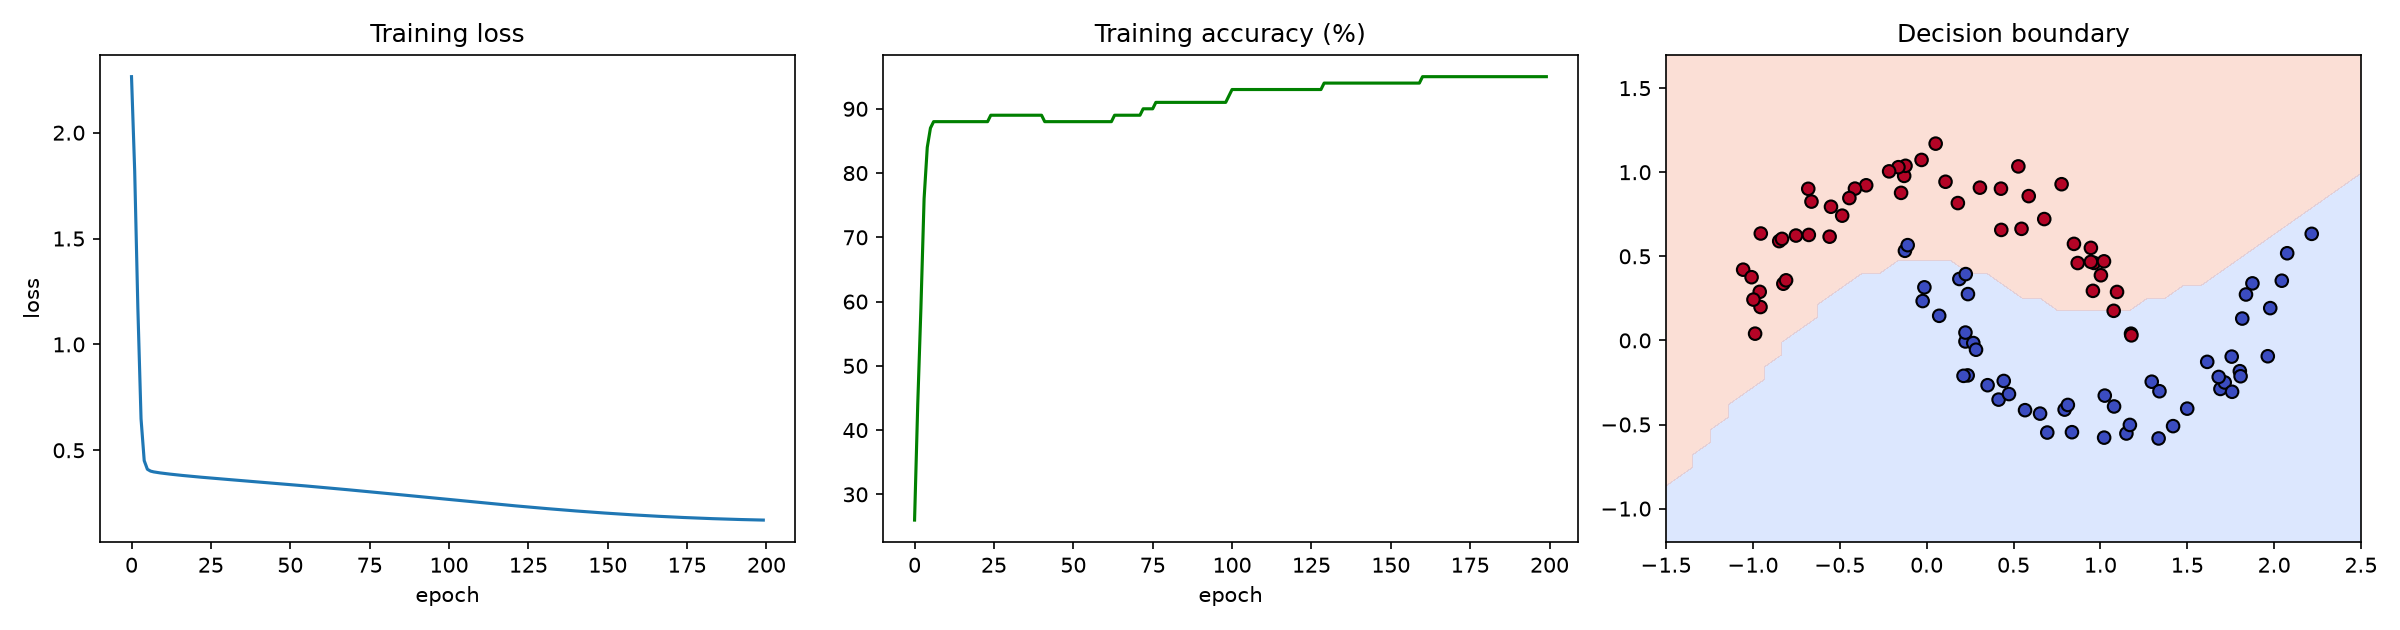
\includegraphics[width=\textwidth]{figures/results.png}
\caption{Training loss, training accuracy and learned decision boundary.}
\end{figure}

The loss falls from $2.26$ to $0.17$ and training accuracy rises from $26\%$ to $95\%$ (final loss $0.1703$).

\paragraph{Observation: tanh saturation.} In a first attempt with \texttt{MLP(2,[16,16,1])} and a learning rate of $0.5$ the run got stuck at loss $\approx2.01$ and $50\%$ accuracy. A loss of $2$ is exactly what a constant output of $+1$ gives on balanced $\pm1$ labels, so the output neuron had saturated. Since $\tanh'(a)=1-\tanh^2(a)\to0$ for large $|a|$, gradients vanish and the network cannot recover. Reducing the learning rate and network width fixed this (a $16\times16$ network with learning rate $0.05$ stalled in the same way in a tuning run, confirming that it was the wide layers with $U(-1,1)$ initialization, whose pre-activations grow with fan-in, that saturated). This illustrates why initialization scale and learning rate matter for saturating activations.

\section{Conceptual Questions}
\paragraph{Q1. Why is a topological sort needed?}
The gradient of a node is the sum over all of its consumers. It is final only after all consumers have run their backward step. A reverse topological order guarantees this ordering; an arbitrary order (e.g.\ creation order of a traversal that visits nodes twice) can use incomplete gradients.

\paragraph{Q2. Why \texttt{+=} instead of \texttt{=} in \texttt{\_backward}?}
A variable used more than once (e.g.\ $c=a+a$, or a weight shared across samples) receives one contribution per use. Assignment would keep only the last one. With \texttt{+=}, $\partial(a+a)/\partial a=2$ is obtained correctly.

\paragraph{Q3. Why must \texttt{zero\_grad()} be called each step?}
For the same reason: gradients accumulate across calls to \texttt{backward()}. Without resetting, each update would use the sum of all previous gradients.

\paragraph{Q4. Forward versus reverse mode.}
Forward mode computes one directional derivative per pass (cost $\propto$ number of inputs for a full gradient); reverse mode computes the gradient of one scalar output with respect to \emph{all} inputs in one backward pass (cost $\approx$ a small constant times the forward pass). Networks have millions of parameters and one scalar loss, so reverse mode (backpropagation) is the efficient choice.

\paragraph{Q5. Why does the seed gradient equal 1?}
Because $\partial L/\partial L=1$; it is the starting value of the chain rule from which all other gradients are derived by multiplication with local derivatives.

\paragraph{Q6. Complexity.}
Both the forward and backward passes are $O(V+E)$ in the number of nodes and edges of the graph, because each node is visited exactly once thanks to the \texttt{visited} set; memory is $O(V)$ since every intermediate value and its closure is retained for the backward pass.

\section{Reproducibility}
\begin{lstlisting}[language=bash]
pip install pytest numpy matplotlib nbformat nbconvert ipykernel
python -m pytest -v             # 12 passed
jupyter nbconvert --to notebook --execute demo.ipynb
\end{lstlisting}
The notebook seeds Python's \texttt{random} and NumPy with 42; the demo takes roughly 20--30 seconds.

\end{document}
